\section{Introdução\label{sec:intro}}

\subsection{Motivação\label{subsec:motiv}}

% O que justifica fazer esse trabalho?
% Quem ou o que é beneficiado por esse trabalho?
% qual a importância disso que queremos fazer?

\subsection{Objetivo\label{subsec:obj}}

% O que queremos fazer?
% O que NÃO queremos fazer
% escopo do trabalho

\subsection{Organização do Texto\label{subsec:org_texto}}


\subsection{Tema}


%Comentário
\begin{comment}
Falar do que se trata o trabalho usando uma visão macroscópica.

Sobre que grande área de conhecimento você vai falar?

Dada esta grande área, qual é o subconjunto de conhecimento sobre o qual será o seu trabalho?

Qual o problema a ser resolvido?
\end{comment}


O tema do trabalho é avaliar o quão saudável uma refeição individual é. Para isso vamos definir uma medida relativa a qualidade de um prato, que pode ser calculada diretamente a partir de seus ingredientes, e cujo valor deverá ser inferido a partir da imagem do próprio prato. Para isto serão empregadas técnicas de visão computacional e aprendizado de máquina. Estas técnicas serão combinadas em um aplicativo para dispositivos móveis, que tornará o processo de avaliação nutricional de refeições diárias mais rápido e prático.


\subsection{Delimitação}


%%%%Comentário

\begin{comment}
Realizar uma delimitação informando de quem é a demanda, em que local, e em que momento no tempo. Eventualmente, pode ser mais fácil começar pensando por exclusão, ou seja, para quem não serve, onde não deve ser aplicado, e em seguida pegar o universo que sobra.
\end{comment}

O funcionamento do aplicativo será baseado em imagens obtidas a partir da câmera do dispositivo móvel. Dessa forma, o desempenho do aplicativo dependerá da qualidade da câmera do aparelho. É importante ressaltar que o aplicativo não se propõe a fazer uma análise nutricional detalhada, como faria um profissional da área. As funcionalidades a serem implementadas serão baseadas em exemplos de refeições previamente analisadas. Sendo assim, sua utilidade será limitada a outras refeições nos mesmos moldes destes exemplos, os quais não contemplam refeições coletivas ou dispostas de forma incomum.


\subsection{Justificativa}
%%%%ler o comentário
\begin{comment}
Apresentar o porquê do tema ser interessante de ser estudado. Cuidado, não é a motivação particular. Devem ser apresentadas razões para que alguém deva se interessar no assunto, e não quais foram suas razões particulares que motivaram você a estudá-lo.
\end{comment}


%MOTIVO 1: MELHORIA DA VIDA HUMANA
A tecnologia sempre esteve presente na vida dos seres humanos. Com o passar dos anos, foram criadas mais e mais ferramentas para tornar nossas vidas mais práticas. Com estas ferramentas podemos facilitar muito nossas atividades. É impossível negar a utilidade dos telefones móveis. Podemos nos comunicar, cuidar da nossa saúde, trabalhar, entender o mundo a nossa volta e alcançar nossas metas.%TODO: A ÙLTIMA FRASE DESTE PARÀGRAFO PARECE FORA DO CONTEXTO. CABE VERIFICAR.

Para tratar as mais distintas necessidades humanas, aplicativos para celular estão sendo desenvolvidos, de forma personalizada. Existem aplicativos para controle de finanças, os que auxiliam no controle de dietas, os que ajudam a controlar os estudos e muitos outros mais. Embora não seja recomendado passar horas utilizando o celular, é sim uma boa ideia saber usá-lo da melhor forma possível.

%MOTIVO 2: UTILIDADE DE APPS SIMILARES
Aplicativos de contagem de calorias são uma das ferramentas que surgiram com o advento de aplicativos que auxiliam no registro e controle das refeições diárias. Eles são recomendados para quem quer controlar a ingestão de calorias, seja para emagrecer ou acompanhar alterações específicas da dieta. Os aplicativos ajudam a ter uma visão ampla e clara de como está sua alimentação \cite{payne2015behavioral}. Assim, é possível fazer ajustes para alcançar determinados objetivos. 

%MOTIVO 3: POSSIBILIDADE DE MELHORIA DE APPS EXISTENTES
A grande maioria desses aplicativos utiliza um filtro de busca através do qual conseguimos pesquisar cada componente da refeição e adicionar as quantidades desejadas. Porém, colocar um alimento por vez, torna a tarefa de contabilizar calorias demorada e nada prática. Entretanto nosso aplicativo busca atacar esse problema de forma diferente.

%Neste sentido, o presente projeto busca aprimorar essa contagem utilizando a câmera do dispositivo. Basta apontar a câmera do dispositivo para a sua refeição e tirar uma foto.

Neste sentido, o presente projeto busca aprimorar essa inserção de alimentos manualmente utilizando a câmera do dispositivo. Basta apontar a câmera do dispositivo para a sua refeição e tirar uma foto. 

Além disso, o projeto se propõe a avaliar uma refeição usando apenas informações visuais, buscando assim não se ater a considerar calorias ou outros valores nutricionais básicos, e também limitar-se a alimentos previamente registrados.


\subsection{Objetivos}

%%comentário
\begin{comment}
Informar qual é o objetivo geral do trabalho, isto é, aquilo que deve ser atendido e que corresponde ao indicador inequívoco do sucesso do seu trabalho. Pode acontecer que venha a existir um conjunto de objetivos específicos, que complementam o objetivo geral (tamanho do texto: livre, mas cuidado para não fazer uma literatura romanceada, afinal esta seção trata dos objetivos).
\end{comment}


Já existem no mercado alguns aplicativos que se propõem a identificar comidas e mostrar seus dados nutricionais.
Em alguns testes com um dos mais robustos, o Calorie Mama \cite{caloriemama_2016}, verificamos que podemos tirar foto do prato e, assim, ele nos mostra opções que se pareçam mais relevantes dados os alimentos que estão no prato, como mostra a Figura \ref{fig:test}.

Diferentemente dos aplicativos que estão no mercado, o objetivo deste trabalho é o desenvolvimento um aplicativo que permita avaliar quão saudável uma refeição individual é utilizando apenas uma imagem do prato. Através de reconhecimento de padrões, baseado num amplo banco de imagens de pratos de refeições com suas respectivas informações nutricionais, será possível informar se o prato é ou não saudável possivelmente considerando atributos como variedade de elementos no prato, coloração do prato, além de outras características ocultas, inferidas a partir de exemplos de fotos de refeições cujos ingredientes e outras informações foram indicadas manualmente \cite{nasrabadi2007pattern}.


\begin{figure}[!ht]
\centering
\caption{Comparação entre diferentes pratos.}
\begin{subfigure}{0.4\textwidth}
  \centering
    \caption{Prato com comidas japonesas.}
   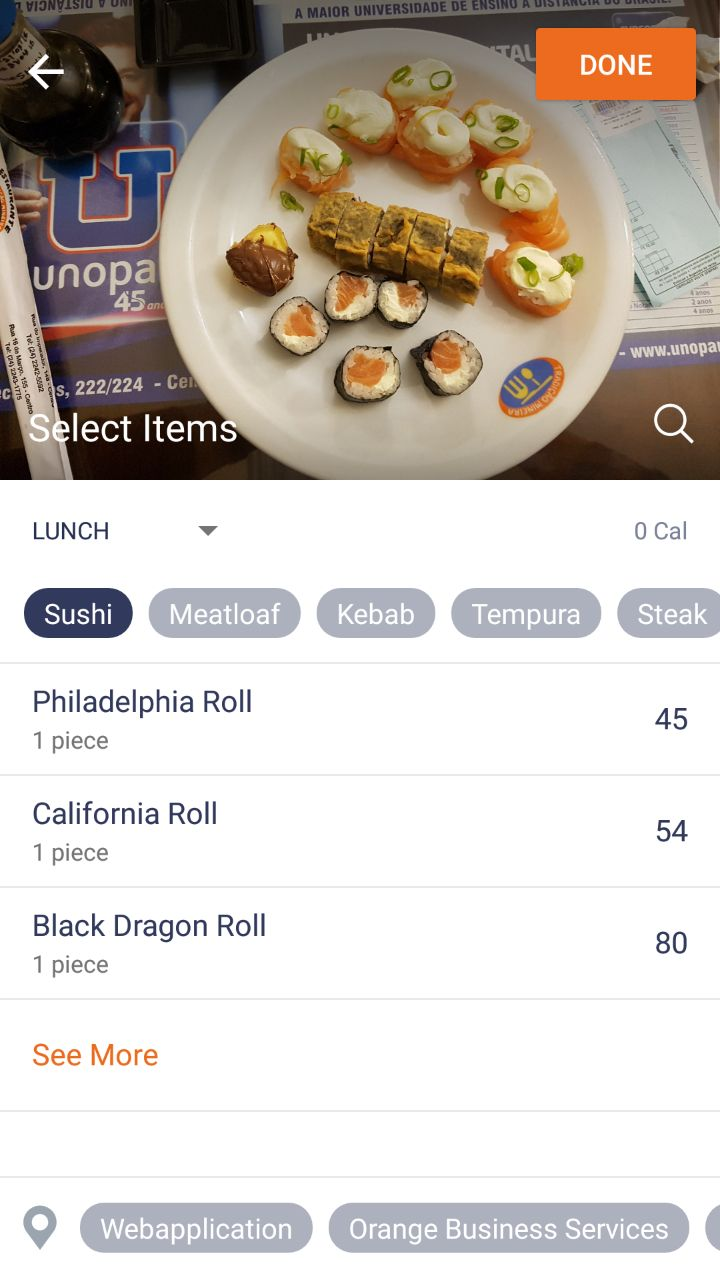
\includegraphics[width=\textwidth]{imgs/sushi.jpeg}
  \label{fig:sub1}
\end{subfigure}%
\hspace{.1\textwidth}
\begin{subfigure}{0.4\textwidth}
  \centering
    \caption{Prato com comidas brasileiras.}
  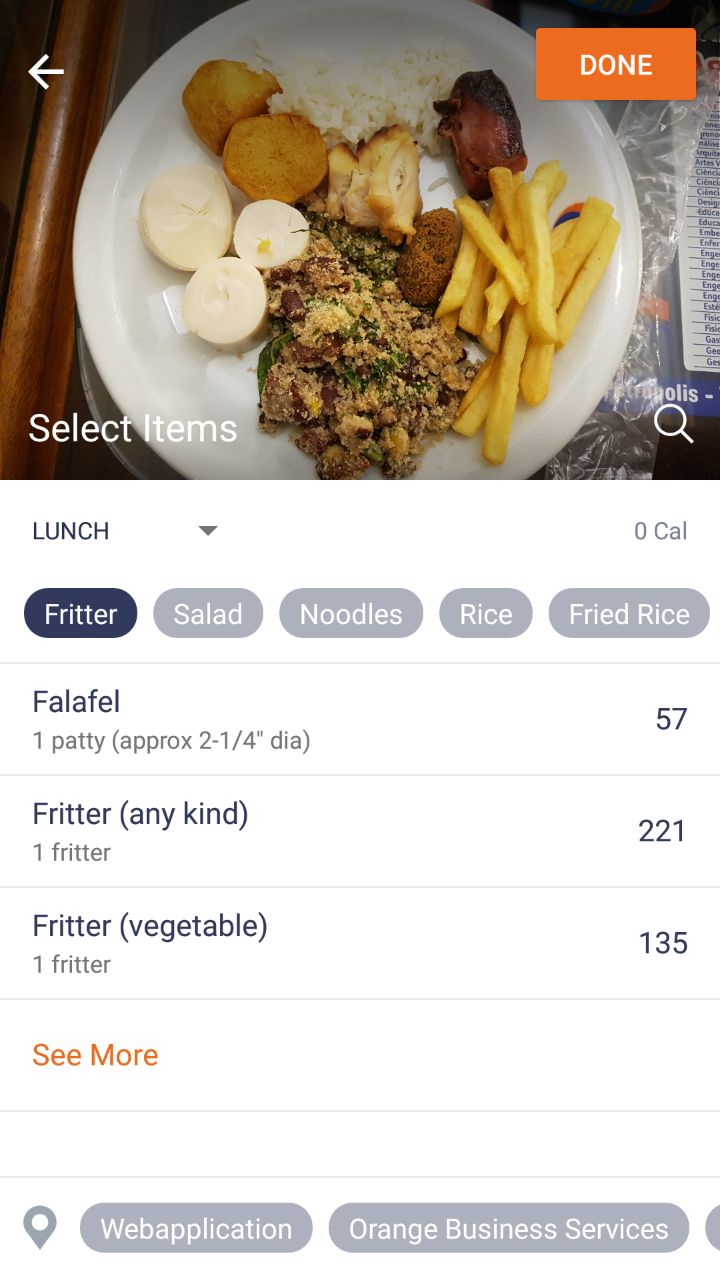
\includegraphics[width=\textwidth]{imgs/brasileira.jpeg}
  \label{fig:sub2}
\end{subfigure}

\label{fig:test}
\end{figure}



\subsection{Metodologia}

%%% comentário
\begin{comment}
Como é a abordagem do assunto. Como foi feita a pesquisa, se vai houve validação, etc. Em resumo, você de explicar qual foi sua estratégia para atender ao objetivo do trabalho.
\end{comment}

Para o aplicativo móvel, implementaremos uma interface simples e de fácil entendimento ao usuário final. Escolhemos o React-Native \cite{react-native_2015} pois permite o desenvolvimento simultâneo para Android e iOS, os sistemas operacionais que dominam o mercado de dispositivos móveis. 

Utilizaremos redes neurais treinadas usando conjuntos de dados com dezenas de milhares de imagens de refeições \cite{kawano2014food}. Por se tratar de um problema com muitas dimensões a serem consideradas, é necessário um grande conjunto de treinamento. Esses conjuntos de dados já estão anotados, contendo indicações de informações dos alimentos presentes na fotografia. Não é necessário se preocupar em ruídos na imagem, como a superfície na qual o objeto se encontra, talheres e o próprio prato. É esperado que o método de aprendizado descarte esses detalhes.
Ao reconhecer o alimento, determinaremos algumas informações nutricionais e outras medidas, como quão colorido é o prato, para podemos informar de alguma forma se o prato é saudável ou não.

\subsection{Organização do texto}

No capítulo 2 será apresentada a base para o estudo de leitura labial, e 

O capítulo 3 apresenta ...

Os .... são apresentados no capítulo 4. Nele será explicitado ...

E assim vai até chegar na conclusão.
